\documentclass[xcolor={usenames,dvipsnames}]{beamer}
\usepackage[utf8x]{inputenc}

\mode<presentation>
{
  \usetheme{Singapore}
  \usecolortheme{rose}
  %\setbeamercovered{transparent}
  \setbeamercovered{invisible}
  \setbeamercolor*{alerted text}{parent=titlelike}
}
\renewcommand{\emph}[1]{\alert{#1}}


%%% Packages %%%

% Use T1 and a modern font family for better support of accents, etc.
\usepackage[T1]{fontenc}
\usepackage{palatino}  % Palatino

% Language support
\usepackage[english]{babel}

% Support for easily changing the enumerator in
% enumerate-environments.
\usepackage{enumerate}

% Support for importing images
%\usepackage{graphicx}

% Use hyperlinks
\usepackage{hyperref}

% Don't load xcolors package in beamer: use document class option
% instead...
%\usepackage[usenames,dvipsnames]{xcolor}

% Use colors in tables
%\usepackage[pdftex]{colortbl}

% My personal list of commonly used math packages and macros
\usepackage{mathcommon}

% More math symbols (e.g. double-brackets: \llbracket, \rrbracket)
%\usepackage{stmaryrd}

% A nice monospace font for listings, etc.
\usepackage[scaled]{beramono}
%\usepackage{inconsolata}

\colorlet{Insertion}{NavyBlue}
\colorlet{Modification}{ForestGreen}
\colorlet{VariableEdge}{Cyan}
\colorlet{SelectorEdge}{Plum}


% Scala listings.  Use colored Scala style by default.
\usepackage{lstscala}
\lstset{
  style=scala-color,
  basicstyle=\footnotesize\tt,
  otherkeywords={do,od},
  moredelim=**[is][\color{Insertion}]{@}{@},
  moredelim=**[is][\color{Modification}]{>}{<}}
\lstnewenvironment{lstscalasmall}{%
  \lstset{style=scala-color,basicstyle=\scriptsize\tt}}{}

% Algorithms/pseud-ocode typesetting
%\usepackage[ruled,vlined,linesnumbered]{algorithm2e}
%\usepackage[slide,vlined,linesnumbered]{algorithm2e}
%\usepackage{float}

% Using TikZ for diagrams
\usepackage{tikz}
\usetikzlibrary{arrows,fit,matrix,positioning}
% Don't use externalize with gradients!!!
%\usetikzlibrary{external,arrows,fit,matrix,positioning}
%\tikzexternalize % Activate externalizing TikZ graphics.

% Support per-slide PGF/TikZ keys (http://tex.stackexchange.com/a/6155)
\tikzset{onslide/.code args={<#1>#2}{%
  \only<#1>{\pgfkeysalso{#2}} % \pgfkeysalso doesn't change the path
}}

\newcommand{\TODO}[1]{\texttt{\textcolor{YellowOrange}{(#1)}}}

%%%% Custom macros %%%%
\newif\ifcompileTreeSlides
%\compileTreeSlidesfalse
\compileTreeSlidestrue

%%% Document info %%%

\title{Solving Shape-Analysis Problems in Languages with Destructive Updating}

\subtitle{SAV Presentation}

\author[Sagiv~et~al.]{%
  {\small Authors}\\ \vspace{1ex}
  Shmuel Sagiv, Thomas W. Reps, Reinhard Wilhelm \\
  \vspace{1em}
  {\small Presenters}\\ \vspace{1ex}
  Marco Antognini, Sandro Stucki
}

% \institute[LAMP, Oracle]{%
%   \inst{1} LAMP, EPFL \and%
%   \inst{2} Oracle Labs}

% Logos
% \logo{
%   \includegraphics[height=7mm]{somelogo.png}\hspace{1mm}
%   \includegraphics[height=7mm]{someotherlogo}
% }

% To show the TOC at the beginning of each section, uncomment this:
% \AtBeginSection[]
% {
%   \begin{frame}<beamer>{Outline}
%     \tableofcontents[currentsection]
%   \end{frame}
% }

% To show the TOC at the beginning of each subsection, uncomment this:
% \AtBeginSubsection[]
% {
%   \begin{frame}<beamer>{Outline}
%     \tableofcontents[currentsection,currentsubsection]
%   \end{frame}
% }


% To uncover everything in a step-wise fashion, uncomment this:
% \beamerdefaultoverlayspecification{<+->}

\setbeamertemplate{footline}[frame number]

\date{%
  \vspace{-1em}
  \small May 2015\\[2em]
  
\includegraphics[height=7mm]{img/epfl-logo}}


%%% Start of the actual document %%%

\begin{document}

\begin{frame}
  \titlepage
\end{frame}

% Short-cut for inline listings using "@" (must come after "\titlepage")
\lstMakeShortInline[%
  style=scala-color,%
  flexiblecolumns=false,%
  mathescape=false,%
  basicstyle=\color{blue!30!darkgray}\tt]@


% No outline, too short a talk...
% \begin{frame}{Outline}
%   \tableofcontents
%   % You might wish to add the option [pausesections]
% \end{frame}

% No sections or subsections, too short a talk...
% \section{Motivation}
% \subsection*{}

\begin{frame}[fragile]{Motivation}
  Analyse the shape of heap allocated data structure

  \vspace{1em}
  
  Verify that a program preserves shape properties such as
  \begin{itemize}
  \item "list-ness"
  \item "circular list-ness"
  \item "tree-ness" \TODO{is it actually supported???}
  \end{itemize}
\end{frame}

\begin{frame}[fragile]{List Reversal: Normalisation}
  \begin{columns}[T]
	  \column{.5\textwidth}
	  \begin{onlyenv}<1>
	  \begin{lstlisting}[mathescape=true]
	  // x point to an unshared list
	  y := nil
	  while x $ \neq $ nil do
	  
	    t := y
	    
	    y := x
	    
	    
	    
	    x := x.cdr
	    
	    y.cdr := t
	  od
	  
	  t := nil
	  \end{lstlisting}
	  \end{onlyenv}
	  \pause
	  
	  \begin{lstlisting}[mathescape=true]
	  // x point to an unshared list
	  y := nil
	  while x $ \neq $ nil do
	    @t := nil@
	    t := y
	    @y := nil@
	    y := x
	    @t$\color{Insertion}_1$ := nil@
	    @t$\color{Insertion}_1$ := x.cdr@
	    @x := nil@
	    >x := t$\color{Modification}_1$<
	    @y.cdr := nil@
	    y.cdr := t
	  od
	  @t$\color{Insertion}_1$ := nil@
	  t := nil
	  \end{lstlisting}
	  
	  \TODO{properly align codes}
	  
	  \column{.5\textwidth}
	  \TODO{Fig 1. (c)}
  \end{columns}
\end{frame}


%%%% The following is a crazy TikZ slide combining tree/graph drawing
%%%% code, etc.

\newcommand{\celldraw}[1]{#1!80!black!80!white}%
\newcommand{\cellfill}[1]{#1!80!black!30!white}%

% Basic style of a cell box.
\tikzstyle{cellbox}=[rectangle, thick, draw=\celldraw{#1}, top color=white,%
  bottom color=\cellfill{#1}, minimum width=2em, minimum height=1em,
  inner sep=0]

% The matrix style underlying graphs.
\tikzstyle{graph}=[matrix, row sep=1pt, column sep=.5em, node distance=0pt,%
  nodes={anchor=center}]

% Basic style for variable labels.
\tikzstyle{labelnode}=[font=\tiny, node distance=.6em, inner sep=1pt]

% Basic cell.  The first argument is the name of the node (in TeX,
% e.g. "xy"), the second one is its printed name (e.g. "n_{x, y}").
% The third argument determines the color.  The optional argument
% contains extra node parameters (e.g. minimum width=1em creates cell
% that is less wide).
\newcommand{\cell}[4][]{%
  \node[rectangle, cellbox=#4, #1] (#2) {};% (#2-car)
  \draw[draw=\celldraw{#4}, semithick] (#2.north) -- (#2.south);
  \path (#2.west) -- coordinate[midway] (#2-car) (#2.center);%
  \path (#2.east) -- coordinate[midway] (#2-cdr) (#2.center);%
  \node[font=\tiny, below=of #2.south west, anchor=north west, inner sep=1pt]
  {$#3$};}%

% A basic cons cell with a circle in the "cdr" box.  Arguments are the
% same as for \cell.
\newcommand{\cons}[4][]{%
  \cell[#1]{#2}{#3}{#4}%
  \node[circle, fill=black, inner sep=.75pt] at (#2-cdr) {};}%

% A concrete (green) cons cell.
\newcommand{\ccons}[3][]{\cons[#1]{#2}{#3}{green}}

% An abstract (blue) cons cell.
\newcommand{\acons}[3][]{\cons[#1]{#2}{n_{#3}}{blue}}

% A shared (red) cons cell.
\newcommand{\scons}[3][]{\cons[#1]{#2}{n_{#3}}{red}}

% Variable label and edge. Arguments are position, node and label text.
\newcommand{\vlabel}[3]{%
  \node[labelnode, #1=of #2] {$#3$} edge (#2);}%

\ifcompileTreeSlides



\begin{frame}[fragile]{Shape-Graph $SG = \langle E_v, E_s \rangle$}

	\textit{Not} to be confused by a program control flow graph $G = (V, A)$
	
	%\begin{center}
	%$ SG \neq G $
	%\end{center}
	
	\vspace{1em}
	What is a \textbf{shape-graph}?
	
	\begin{itemize}
	\item directed graph with nodes and edges
	\item nodes are called \textcolor{Green}{\textbf{shape-nodes}}
		\begin{itemize}
		\item[$\circ$] runtime locations, i.e. heap memory, or \textit{cons-cells}
		\item[$\circ$] implicitly defined by edges and $shape\_nodes(SG)$
		\end{itemize}
	\item edges are divided into 2 categories:
		\begin{itemize}
    	\item[$\circ$] \textcolor{VariableEdge}{$E_v$: \textbf{variable-edges}} of the form $ \left[x, n\right] $
    	\item[$\circ$] \textcolor{SelectorEdge}{$E_s$: \textbf{selector-edges}} of the form $ \langle s, sel, t \rangle $
		\end{itemize}
	\end{itemize}
	
	\begin{center}
    \begin{tikzpicture}[semithick,
      ampersand replacement=\&, every edge/.append style={->}, >=latex]
      \Large % <-- determines scale of diagram. try \LARGE, \Huge, \small...

      % Matrix for arranging graph nodes.  You can set the overall
      % spacing through "row sep" and "column sep" or add and remove
      % horizontal or vertical space in brackets after \& and \\.
      \matrix[graph, column sep=1em] (g1) %<-- general column spacing
      {
        \ccons[minimum width=1em]{l1}{l_1} \&
        \ccons[minimum width=1em]{l2}{l_2} \&
        \ccons[minimum width=1em]{l3}{l_3} \\
      };

      % Selector edges.
      \path[->]
      (l1-cdr) edge[SelectorEdge] (l2)
      (l2-cdr) edge[SelectorEdge] (l3);

      % Variable egdes.
      %\vlabel{left}{l1}{x} % need color on edge:
      \node[labelnode, left=of l1] {$x$} edge[VariableEdge] (l1);
    \end{tikzpicture}
  \end{center}
	
	$n, s, t, l_1, l_2$ and $l_3$ are shape-nodes, $x$ a program variable and $sel \in \left\{ car, cdr \right\}$

\end{frame}



\begin{frame}[fragile,t]{Graph example}
  \vspace{-0.5em}\uncover<2-4>{ % this diagram is visible in slides 2-4.
  \begin{center}
    \begin{tikzpicture}[semithick,
      % The "level X" styles below can be used to uncover graphs or
      % parts thereof across slides.
      level 2/.style={onslide=<-2>{transparent}},
      level 3/.style={onslide=<-3>{transparent}},
      ampersand replacement=\&, every edge/.append style={->}, >=latex]
      \Large % <-- determines scale of diagram. try \LARGE, \Huge, \small...


      % Matrix for arranging graph naodes.  You can set the overall
      % spacing through "row sep" and "column sep" or add and remove
      % horizontal or vertical space in brackets after \& and \\.
      \matrix[graph, column sep=1em] (g1) %<-- general column spacing
      {
        \ccons[minimum width=1em]{l1}{l_1} \&
        \ccons[minimum width=1em]{l2}{l_2} \&[-.5em] % <-- remove space
        \ccons[minimum width=1em]{l3}{l_3} \\
      };

      % Selector edges.
      \path[->]
      (l1-cdr) edge (l2)
      (l2-cdr) edge (l3);

      % Variable egdes.
      \vlabel{left}{l1}{x}

      % This second graph won't be shown until slide 3.
      \begin{scope}[yshift=-4em, level 2]
        \matrix[graph] (g2) %
        {
          \acons{x}{\{x\}} \& \\
          \acons{xt1}{\{x, t_1\}} \&
          \scons{e}{\emptyset}\\[.5em] % <-- extra space
          \acons{y}{\{y\}} \& \acons{t}{\{t\}}\\
        };

        % Selector edges.
        \path[->] % Normal edges.
        (x-cdr) edge (e.north west)
        (xt1-cdr) edge (e)
        (y-cdr) edge (t);
        % A loop.  Not visible until slide 4.
        \draw[->, level 3] (e-cdr) -| ++(1em, 1em) -| (e.north);

        % Variable egdes.
        \vlabel{left}{x}{x}
        \vlabel{yshift=1ex,left}{xt1}{x}
        \vlabel{yshift=-1ex,left}{xt1}{t_1}
        \vlabel{left}{y}{y}
        \vlabel{right}{t}{t}
      \end{scope}
    \end{tikzpicture}
  \end{center}}
  The diagram above won't show up until slide 2.
\end{frame}
\fi

\begin{frame}[fragile]{Some citations and maths}
  The \emph{Probability Monad} is a variant of the @List@
  monad.\footnote{See e.g.\ \cite{RamseyP2002popl,Gibbons2012utp}}

  \begin{lstlisting}
  type Dist[+A] = List[(A, Double)]
  final case class Rand[+A](dist: Dist[A]) {
    // Monadic "bind"
    def flatMap[B](f: A => Rand[B]): Rand[B] = Rand(
      for ((v, p) <- dist; (w, q) <- f(v).dist)
      yield (w, q * p))
    ...
  }
  \end{lstlisting}
  Computations are sequenced using the \emph{chain rule}:
  \[
  \Pr\{ f(X) = y \} = \sum_{x} \Pr\{ f(X) = y \,|\, X = x \} \Pr\{ X =
  x \}
  \]
\end{frame}

\begin{frame}{Thank you!}
  \begin{center}
    \Huge Questions?
  \end{center}
\end{frame}

%%%  Backup slides  %%%

\appendix
\newcounter{finalframe}
\setcounter{finalframe}{\value{framenumber}}

\begin{frame}[noframenumbering]
  \begin{center}
    \emph{\LARGE Additional slides}
  \end{center}
\end{frame}

\begin{frame}[fragile]{The \texttt{grassModel} in Odds}
  \setcounter{framenumber}{\value{finalframe}}%
  \begin{lstlisting}
  trait CodeExample extends Stuff {
    def grassModel: Rand[Boolean] = {
      val rain       = flip(0.3)
      val sprinkler  = flip(0.5)
      val grassIsWet =
        flip(0.9) && rain      ||
        flip(0.8) && sprinkler ||
        flip(0.1)
      if (grassIsWet) rain else never
    }
  }
  \end{lstlisting}
\end{frame}

\begin{frame}[noframenumbering]{Quotes and graphics}
  The Monty Hall problem:
  \begin{quote}
    Suppose you're on a game show, and you're given the choice of
    three doors: Behind one door is a car; behind the others,
    goats. You pick a door, say No. 1, and the host, who knows what's
    behind the doors, opens another door, say No. 3, which has a
    goat. He then says to you, "Do you want to pick door No. 2?" Is it
    to your advantage to switch your choice?

    \hfill{\em \cite{vosSavant1990monty}}
  \end{quote}
  \begin{center}
    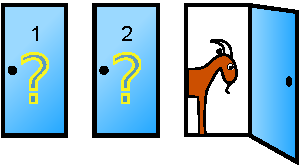
\includegraphics[height=2cm]{img/monty/Monty_open_door}
  \end{center}
\end{frame}


%%% Bibliography

\bibliography{monty,biblio}
\bibliographystyle{apalike}

\end{document}


